\documentclass[11pt]{article} % For LaTeX2e
\usepackage{nips12submit_e,times}
%\documentstyle[nips12submit_09,times,art10]{article} % For LaTeX 2.09

%\usepackage[usenames,dvipsnames]{color}

\usepackage[utf8]{inputenc}
\usepackage[T1]{fontenc}
\usepackage{textcomp}
\usepackage[scaled=0.8]{beramono}

\usepackage{caption}
\usepackage{subcaption}
\usepackage{wrapfig}
\usepackage{amsmath,amssymb}
\usepackage{array}
\usepackage{tabularx}
\usepackage{booktabs}
\usepackage{graphicx}
\usepackage{placeins}

\usepackage{cite}
\usepackage{url}
\usepackage[hyperfootnotes=false,citecolor=RedOrange,linkcolor=RoyalBlue,urlcolor=DarkOrchid,colorlinks]{hyperref}
\usepackage[all]{hypcap}

\newcommand{\todo}[1]{\noindent\texttt{\color[rgb]{0.5,0.1,0.1} TODO: #1}}


\newcommand{\sectref}[1]{\hyperref[#1]{\mbox{Section~\ref*{#1}}}}
\newcommand{\figref}[1]{\hyperref[#1]{\mbox{Figure~\ref*{#1}}}}
\newcommand{\tabref}[1]{\hyperref[#1]{\mbox{Table~\ref*{#1}}}}
\newcommand{\eqtref}[1]{\hyperref[#1]{\mbox{Equation~\ref*{#1}}}}

\newcommand{\argmax}{\operatornamewithlimits{argmax}}
\newcommand{\argmin}{\operatornamewithlimits{argmin}}
\newcommand{\twopartdef}[4]
{
	\left\{
		\begin{array}{ll}
			#1 & \mbox{if } #2 \\
			#3 & \mbox{if } #4
		\end{array}
	\right.
}

\title{Active Learning of Function Contours using Gaussian Process Confidence Bounds\thanks{Final
report for the course \emph{Research in Computer Science} (Spring
Semester 2012), carried out under the supervision of \emph{Prof. Andreas Krause.}}}

\author{
Alkis Gkotovos\\
Department of Computer Science, ETH Zurich\\
\texttt{alkisg@student.ethz.ch}
}

\nipsfinalcopy % Uncomment for camera-ready version

\begin{document}

\maketitle

\begin{abstract}
We present a novel heuristic for actively identifying function
contours using the framework of Gaussian processes to model the underlying
function and utilizing the
inferred confidence bounds to guide the learning process. We also show how
the proposed heuristic can be extended to identify $\epsilon$-optimal function
contours. Our method is evaluated and compared to the state of the art on
synthetic and real-world seismographic data.
\end{abstract}

\section{Introduction}
In certain applications it is required to experimentally determine the regions
where the values of a function are above (or below) a certain threshold.
Furthermore, obtaining measurements of the function is expensive, so it is
important to
accurately determine the desired contours with as few samples as possible.
This suggests using an active learning procedure that selects measurements
over the function domain in a more efficient way than random sampling.

In~\sectref{sect:algo} we formalize the active learning setting,
review the previously proposed \emph{straddle}~\cite{bryan2005} heuristic,
and introduce the confidence bound heuristic, as well as its extension
to the $\epsilon$-optimal setting. In~\sectref{sect:exp} we
evaluate our heuristic on a synthetic function and a real-world seismographic
dataset.

\section{Algorithm} \label{sect:algo}
The problem of actively learning function contours can be described as follows.
Let ${f : \mathcal{D} \to \mathbb{R}}$ be the target function, where
$\mathcal{D}$ is a bounded subset of $\mathbb{R}^n$. We are interested in
finding the subset of $\mathcal{D}$ where this function takes values greater
than a specified threshold $t$, i.e. the set
$\mathcal{G}_t = \{x \in \mathcal{D} \mid f(x) > t\}$. To this end, we take
consecutive measurements $(x^{(i)}, f(x^{(i)}))$ of the function
and use them to determine $\mathcal{G}_t$. After the $i$-th step, the set of
all acquired measurements is
$\mathcal{M}^{(i)} = \{(x^{(1)}, f(x^{(1)})),\ldots,(x^{(i)}, f(x^{(i)}))\}$.

As mentioned before, our basic premise is that the effort required to obtain
each measurement is
non-negligible and, therefore, taking a large number of random measurements
over the whole domain $\mathcal{D}$ is prohibitive. We rather aim at directing
the measurement process so that the chosen points $x^{(i)}$ are informative with
respect to the desired contours, which should result in accurately determining
the set $\mathcal{G}_t$ using a significantly smaller number of measurements
compared to random sampling.

In this setting, we have to decide on (1) a model that allows us to use the
measurements in order to obtain an approximation of $\mathcal{G}_t$, and (2) a
strategy to select the next point of measurement at each step. The following
subsections deal with these two issues.

\subsection{Gaussian processes}
We chose to use Gaussian processes~\cite{gpbook} in modeling the target
function $f$, as they have been successfully used before in the context of
contour detection~\cite{bryan2005, bryan2008}. Gaussian process regression
offers a non-parametric framework for predicting the values of the function at
unobserved points, given a number of measurements. The characteristics of
the assumed underlying model are primarily specified by a kernel function
${K : \mathcal{D} \times \mathcal{D} \to \mathbb{R}}$, which determines the
covariance of any two points in $\mathcal{D}$.

In our active learning setting, $\mathcal{M}^{(i)}$ is used as a training set
for Gaussian process regression and the inferred mean $m^{(i)}(x)$ of the
model is used to approximate the set $\mathcal{G}_t$ as
${\mathcal{G}^{(i)}_t = \{x \in \mathcal{D} \mid m^{(i)}(x) > h\}}$.

\subsection{Choosing the next point}
The general strategy for choosing the next point of measurement at each step $i$
is to first establish a finite set $\mathcal{C}^{(i)} \subseteq \mathcal{D}$ of
candidate points, then evaluate some heuristic
${h : \mathcal{C}^{(i)} \to \mathbb{R}}$ for each candidate point and, finally,
choose the point with the largest heuristic value, that is
\begin{align*}
  x^{(i+1)} = \underset{x \in \mathcal{C}^{(i)}}{\argmax}\{h(x)\}
\end{align*}
If $\mathcal{D}$ is finite, we can use
$\mathcal{C}^{(i)} = \mathcal{D}\setminus\mathcal{M}_i$ or a random subset
thereof in case $\mathcal{C}_i$ is too large. Otherwise, we have to sample a set
of candidate points from $\mathcal{D}$. Random sampling is preferred over a
fixed grid to get better coverage of $\mathcal{D}$~\cite{bryan2005}.

Choosing the heuristic $h$ involves an exploration-exploitation trade-off. The
state of the art in contour detection combines the inferred variance of the
Gaussian process with the
distance from the inferred contour to create the straddle~\cite{bryan2005}
heuristic ${h_{straddle}(x) = 1.96\sigma(x) - | m(x) - t |}$, where $m(x)$
and $\sigma(x)$ are respectively the inferred mean and variance of the Gaussian
process at the candidate point $x$.

\begin{figure}[tb]
  \centering
  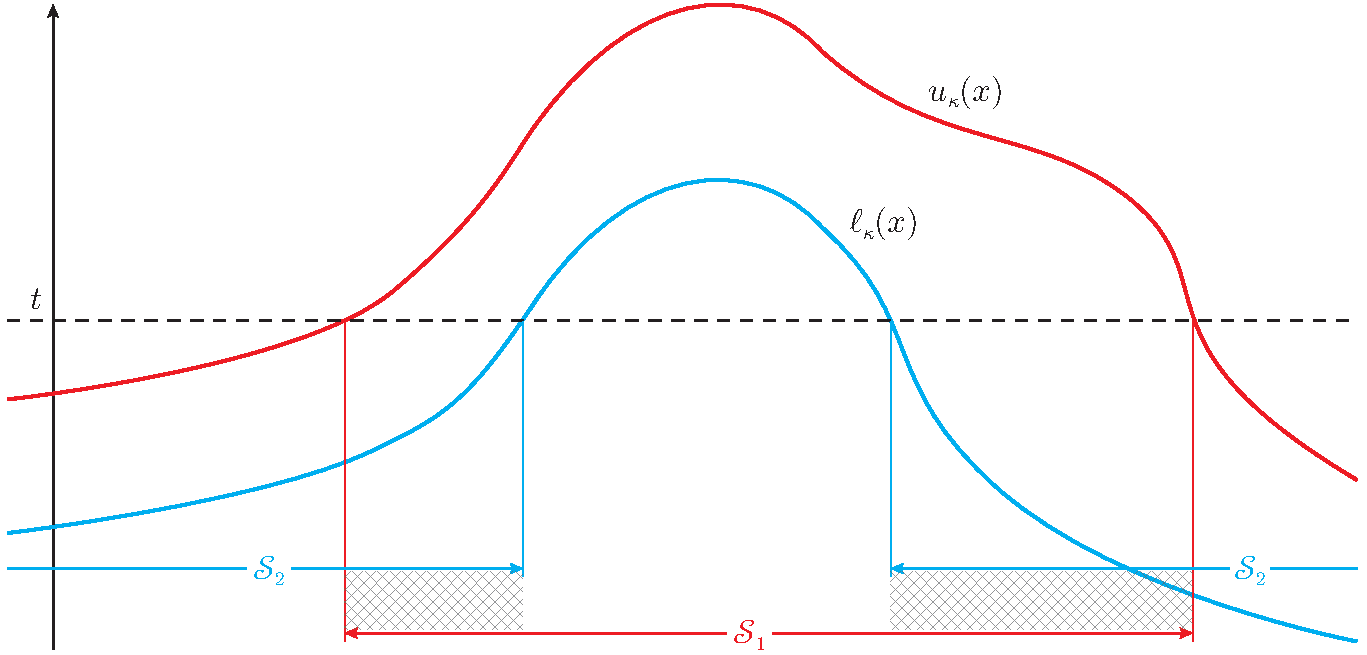
\includegraphics[width=\textwidth]{figures/cb}
  \caption{A one-dimensional example showing the two sets $\mathcal{S}_1$ and
           $\mathcal{S}_2$, as well as the (shaded) confidence region
           $\mathcal{S} = \mathcal{S}_1\cap\mathcal{S}_2$.}
  \label{fig:cb}
  \vspace{-0.5em}
\end{figure}

Our proposed heuristic is based on the fact that we can construct confidence
bounds for the desired contour by using the inferred mean and variance of
the Gaussian process. In particular, for every $x \in \mathcal{D}$ we obtain
a confidence interval ${[m(x) - \kappa\sigma(x), m(x) + \kappa\sigma(x)]}$,
where the probability of $x$ being in the interval depends on the value
of $\kappa$. Extending this idea and defining the functions
$u_{\kappa}(x) = m(x) + \kappa\sigma(x)$ and
$\ell_{\kappa}(x) = m(x) - \kappa\sigma(x)$,
we can create a confidence region for
the desired contour at level $t$ by using two sets
\begin{align*}
  \mathcal{S}_1 &= \{x \in \mathcal{D} \mid u_{\kappa}(x) \geq t\}\\
  \text{and}\hspace{1em}
  \mathcal{S}_2 &= \{x \in \mathcal{D} \mid \ell_{\kappa}(x) \leq t\}
\end{align*}
The confidence region is then
$\mathcal{S} = \mathcal{S}_1\cap\mathcal{S}_2$ (see~\figref{fig:cb}) and our
heuristic is defined
so that the point with the largest variance among the candidate points that
lie inside the confidence region is chosen:
\begin{align}\label{eq:hcb}
  h_{cb}(x) = \twopartdef { \sigma(x) } {x \in \mathcal{S}} {-\infty} {x \notin \mathcal{S}}
\end{align}
In other words, we exlude candidate points in the region where
$f(x) < t$ with high probability (the set $\mathcal{D}\setminus\mathcal{S}_1$)
and in the region where $f(x) > t$ with high probability
(the set $\mathcal{D}\setminus\mathcal{S}_2$).

From the above definitions it follows that 
$\mathcal{D}\setminus\mathcal{S}_2\subseteq\mathcal{S}_1$
and, equivalently, $\mathcal{S}\neq\varnothing$. We can also see that
obtaining more measurements leads to lower variance values, which in turn
generally reduces the size of $\mathcal{S}$.

\subsection{Detecting $\epsilon$-optimal contours}
The confidence bound heuristic described in the previous subsection can be
readily extended for detecting $\epsilon$-optimal function contours,
i.e. for approximating the set
${\mathcal{G}_{\epsilon} = \{x \in \mathcal{D} \mid f(x) > \underset{x \in \mathcal{D}}{\max}\,f(x) - \epsilon\}}$.
In this case, the sets used to define the confidence region $\mathcal{S}$
are defined as
\begin{align*}
  \mathcal{S}_1 &= \{x \in \mathcal{D} \mid u_{\kappa}(x) \geq \underset{x \in \mathcal{D}}{\max}\,\ell_{\kappa}(x) - \epsilon\}\\
  \text{and}\hspace{1em}
  \mathcal{S}_2 &= \{x \in \mathcal{D} \mid \ell_{\kappa}(x) \leq \underset{x \in \mathcal{D}}{\max}\,u_{\kappa}(x) - \epsilon\}
\end{align*}
Using the same confidence region $\mathcal{S} = \mathcal{S}_1\cap\mathcal{S}_2$
as before, runs the risk of exluding areas where the true maximum might lie.
Since the approximation
${\mathcal{G}^{(i)}_\epsilon = \{x \in \mathcal{D} \mid m^{(i)}(x) > \underset{x \in \mathcal{D}}{\max}\,m^{(i)}(x) - \epsilon\}}$
of $\mathcal{G}_{\epsilon}$ at each step
depends on the inferred maximum, it is important to have an accurate estimate
of the true maximum in order to get an accurate approximation of the desired
$\epsilon$-optimal contour. For that reason, we include in $\mathcal{S}$ the
region where the true maximum could still lie with high probability, i.e.
the set
\begin{align*}
  \mathcal{S}_3 &= \{x \in \mathcal{D} \mid u_{\kappa}(x) \geq \underset{x \in \mathcal{D}}{\max}\,\ell_{\kappa}(x)\}
\end{align*}
Therefore, the resulting confidence region is
$\mathcal{S} = \mathcal{S}_1\cap\mathcal{S}_2\cup\mathcal{S}_3$, as shown
in~\figref{fig:cbe}, and the heuristic function is the same as
in~\eqtref{eq:hcb}.

\begin{figure}[tb]
  \centering
  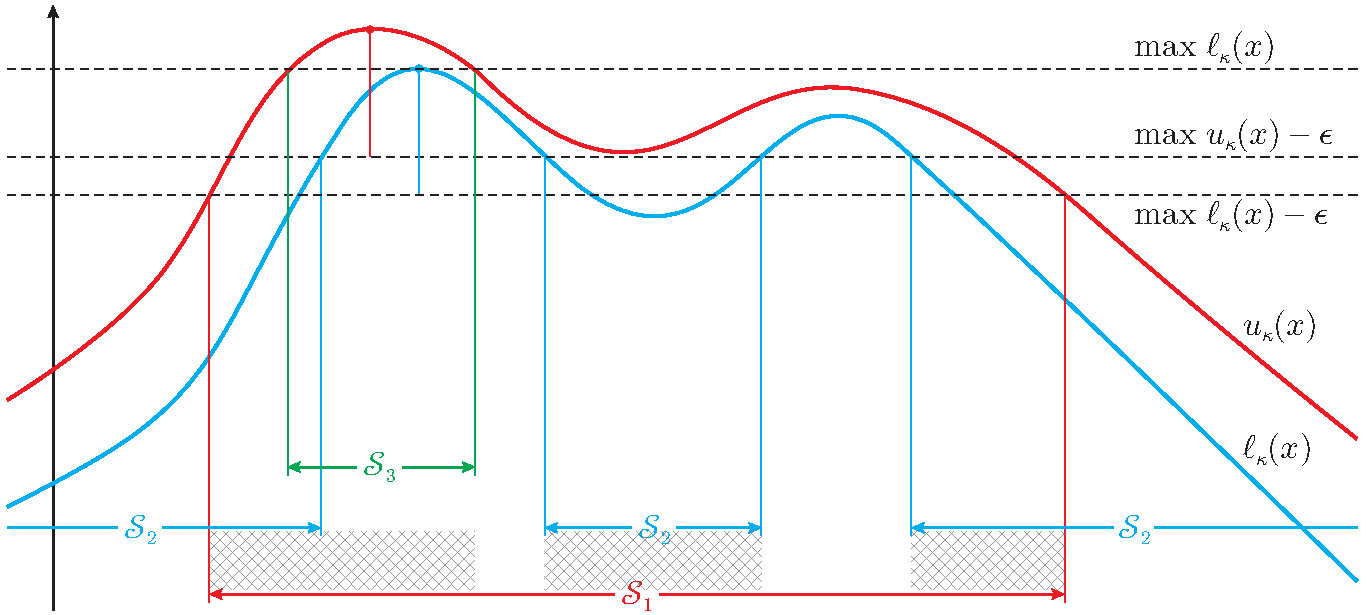
\includegraphics[width=\textwidth]{figures/cb_eps}
  \caption{A one-dimensional example showing the three sets $\mathcal{S}_1$,
           $\mathcal{S}_2$ and $\mathcal{S}_3$, as well as
           the (shaded) confidence region
           $\mathcal{S} = \mathcal{S}_1\cap\mathcal{S}_2\cup\mathcal{S}_3$.}
  \label{fig:cbe}
  \vspace{-0.5em}
\end{figure}

\section{Experiments} \label{sect:exp}
We developed a contour detection framework prototype in Matlab, which uses the
GPML toolbox\footnote{\url{http://www.gaussianprocess.org/gpml/}} for
Gaussian process inference. In short, our framework allows for providing
targets as functions or discrete data sets,
implements the previously described heuristics for contour detection, and
provides contour evaluation and visualization capabilities.

In the following we evaluate our proposed heuristics on two experiments.
The first is carried out on a synthetic two-dimensional sinusoidal target
function proposed by Bryan et al.~\cite{bryan2005} for evaluating the straddle
heuristic. The function is defined as
\begin{align*}
  f(x, y) = \sin(10x) + \cos(4y) - \cos(3xy)
\end{align*}
with domain
$\mathcal{D} = \{(x, y) \in \mathbb{R} \mid 0 \leq x \leq 1,\;0 \leq y \leq 2\}$.
For the second experiment we use a two-dimensional seismographic dataset
collected by about 4089 sensors in California. For the first experiment
we use 1000 uniformly random candidates at each step, while for the second
one every unused sample point is a candidate at each step. For both
experiments $k = 2$.
We first discuss two important issues that came up during evaluation.

\noindent\emph{Kernel and hyperparameters.}\;The choice of the Gaussian process
kernel function and its hyperparameters can have a considerable impact on the
performance of contour detection. In both experiments we use a
Matern-5~\cite{gpbook} kernel function. For the first experiment, we initialize
the algorithm with 20 random measurements and optimize the hyperparameters with
respect to these measurements. Moreover, we re-optimize the hyperparameters at
exponentially increasing measurement-set sizes
(at $20\times 2^n$ samples, $n = 0, 1,\ldots$). This is done to avoid cases
where the initially estimated hyperparameters are not accurate due to bad luck.
On the other hand, re-optimizing the hyperparameters too often is not only
computationally inefficient, but can also lead to worse results.
For the second experiment, we also have a different seismographic dataset
to our disposal, thus we compute appropriate hyperparameters for this other
dataset and use them for our experiment (without re-optimizing).

\noindent\emph{Evaluation metric.}\;We will use three different ``metrics'' to
measure the quality of the inferred contours. The first is classification
accuracy of points being above or below the contour threshold. The second is
by approximating the area of the set $\mathcal{D}\setminus\mathcal{S}$, which is
done by again computing the classification accuracy, but only considering points
outside the confidence region $\mathcal{S}$ as correctly classified.
We will call this metric \emph{strict accuracy} and, intuitively, it measures
the certainty about the inferred contours according to the Gaussian process
model. The third metric is a modified version of the Hausdorff distance, which
is normally defined as
$D_{hd}(\mathcal{X}, \mathcal{Y}) =
\max\{\underset{x\in\mathcal{X}}{\max}\;\underset{y\in\mathcal{Y}}{\min}\;d(x, y),
      \underset{x\in\mathcal{X}}{\max}\;\underset{y\in\mathcal{Y}}{\min}\;d(x, y)\}$,
where $d(x, y)$ is the Euclidean distance between $x$ and $y$.
In our case, $\mathcal{X}$ and $\mathcal{Y}$ consist of a number of points on
the true and inferred contours respectively (as computed by Matlab's
\texttt{contourc}). Furthermore, to mitigate the effect of the inner maxima,
we replace them by $L^{20}$-norms of the corresponding sets converted to
vectors. Finally, we normalize the distance to lie in $[0, 1]$ and subtract it
from 1 in order to get a similarity metric. We call the result
\emph{normalized Hausdorff similarity} metric or NHDS.

\subsection{Experiment 1}
For the first experiment we used a threshold value of $h = 0$.
\figref{fig:sin2d_steps} shows the evolution of the inferred contour and the
confidence region for a single execution of the algorithm using the confidence
bound heuristic. Note how the measurements gather around the true contour
as the confidence region shrinks. In \figref{fig:sin2d_eval} the performance
of our heuristic is compared to the straddle heuristic using the three metrics
presented before. The algorithm was run 20 times for each heuristic and the
errorbars have a height of two standard errors. We also depict the performance
of random sampling as a baseline. The performance of the two heuristics seems
to be comparable, while both are
clearly superior to random sampling. It is also evident that the NHDS metric
distinguishes in this case more clearly than the other metrics between
random sampling and the two heuristics.

We also evaluated the $\epsilon$-optimal conf. bound heuristic on the same
function. The value of $\epsilon$ was chosen so that the desired contour
level be the same as above, i.e.
${\underset{x\in\mathcal{D}}{\max}\;f(x) - \epsilon = 0}$. We expect our algorithm
to be less effective when searching for an $\epsilon$-optimal contour, since
it has to correctly infer an accurate maximum value in order to also infer
an accurate contour. Indeed, the results of~\figref{fig:sin2d_eval_eps} are
slightly worse than the ones of~\figref{fig:sin2d_eval}.

\begin{figure}[tb]
  \begin{subfigure}[b]{0.5\textwidth}
    \centering
    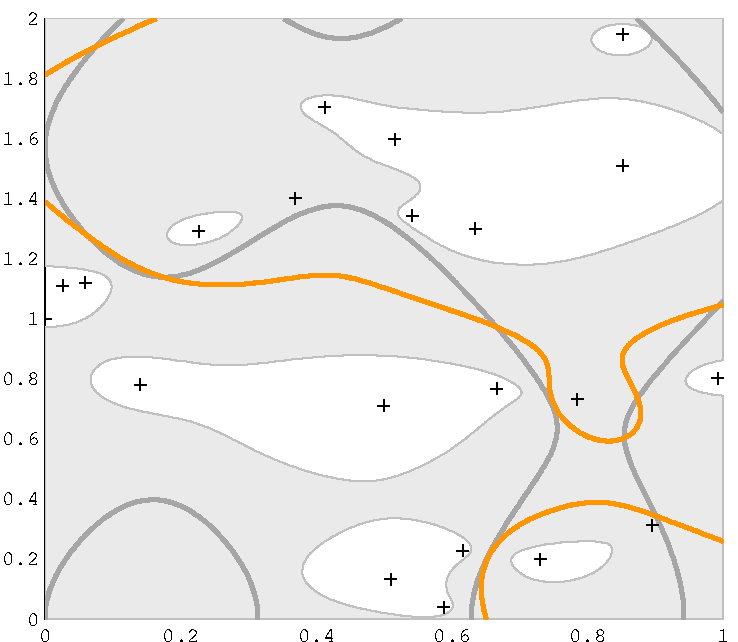
\includegraphics[width=\textwidth]{figures/sin2d_20}
    \caption{20 measurements}
  \end{subfigure}
  \hfill
  \begin{subfigure}[b]{0.5\textwidth}
    \centering
    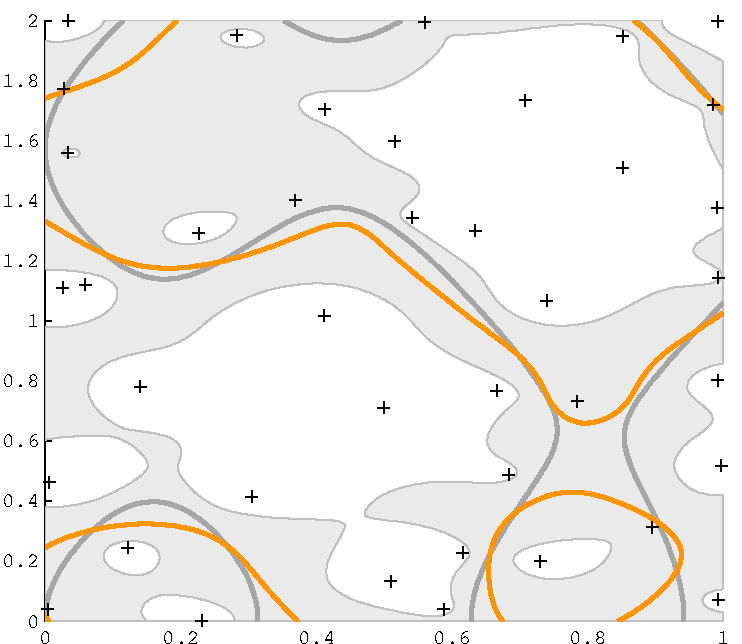
\includegraphics[width=\textwidth]{figures/sin2d_40}
    \caption{40 measurements}
  \end{subfigure}
  \begin{subfigure}[b]{0.5\textwidth}
    \centering
    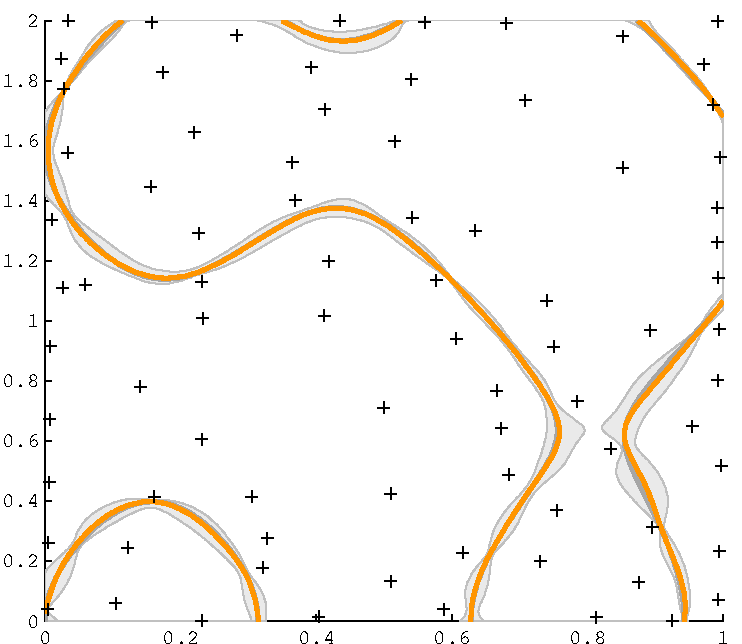
\includegraphics[width=\textwidth]{figures/sin2d_80}
    \caption{80 measurements}
  \end{subfigure}
  \hfill
  \begin{subfigure}[b]{0.5\textwidth}
    \centering
    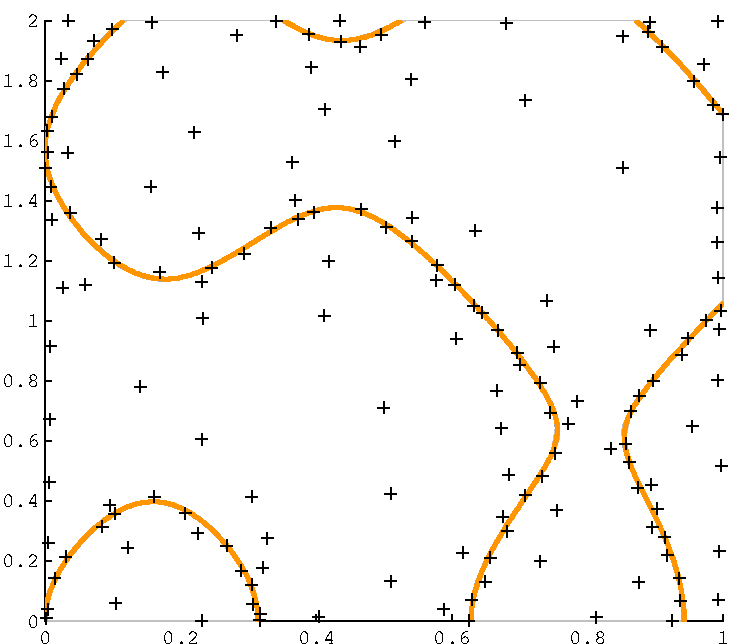
\includegraphics[width=\textwidth]{figures/sin2d_160}
    \caption{160 measurements}
  \end{subfigure}
  \caption{Inferred contour (orange), true contour (dark grey) and confidence
           region $\mathcal{S}$ (light grey) for one execution of the
           contour detection algorithm on the synthetic sinusoidal target
           function using our proposed confidence bound heuristic.}
  \label{fig:sin2d_steps}
\end{figure}

\begin{figure}[tb]
  \begin{subfigure}[b]{0.329\textwidth}
    \centering
    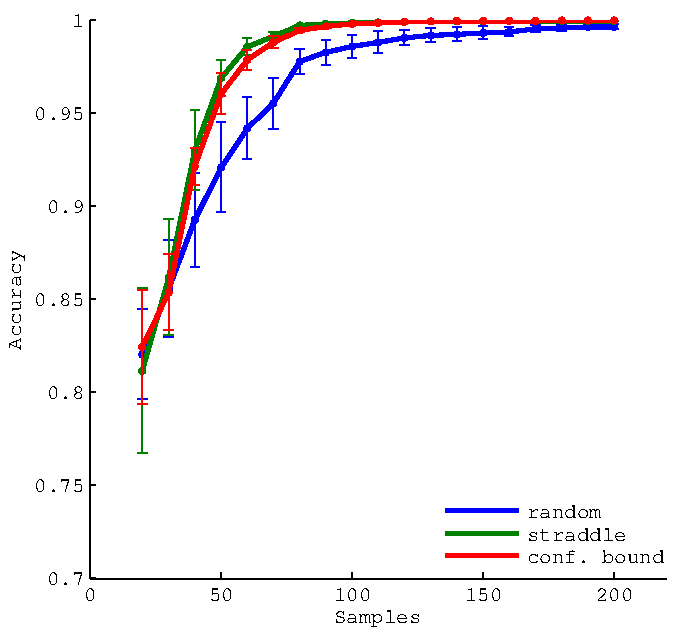
\includegraphics[width=\textwidth]{figures/sin2d_acc}
    \caption{Accuracy}
  \end{subfigure}
  \hfill
  \begin{subfigure}[b]{0.329\textwidth}
    \centering
    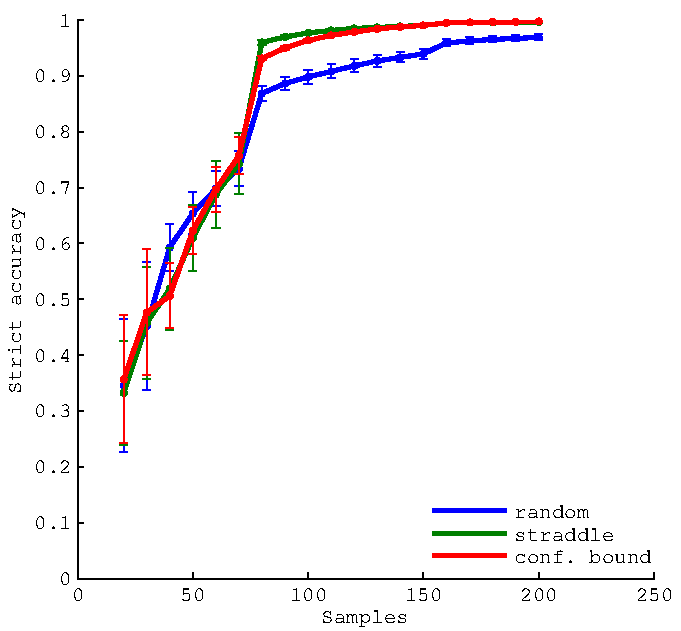
\includegraphics[width=\textwidth]{figures/sin2d_strict_acc}
    \caption{Strict accuracy}
  \end{subfigure}
  \hfill
  \begin{subfigure}[b]{0.329\textwidth}
    \centering
    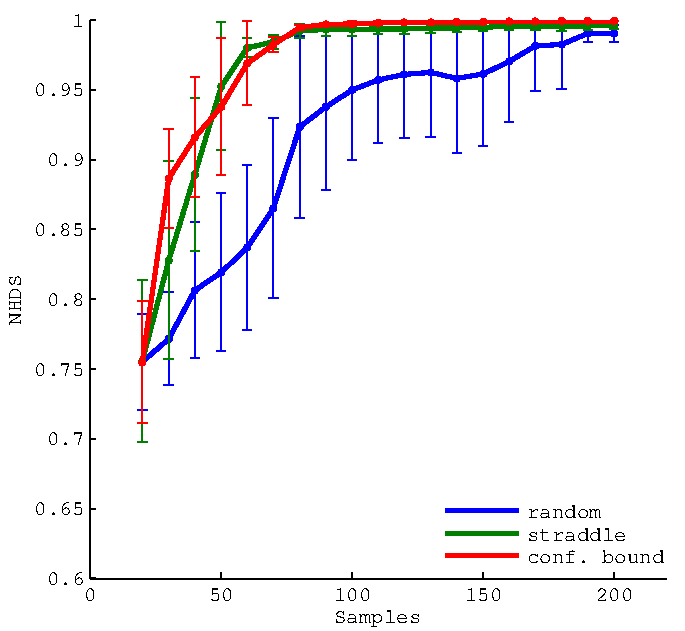
\includegraphics[width=\textwidth]{figures/sin2d_hd}
    \caption{NHDS}
  \end{subfigure}
  \caption{Random, straddle and conf. bound heuristics evaluated on the three
           metrics for an increasing number of measurements
           (Experiment 1, 20 iterations).}
  \label{fig:sin2d_eval}
\end{figure}

\begin{figure}[tb]
  \begin{subfigure}[b]{0.329\textwidth}
    \centering
    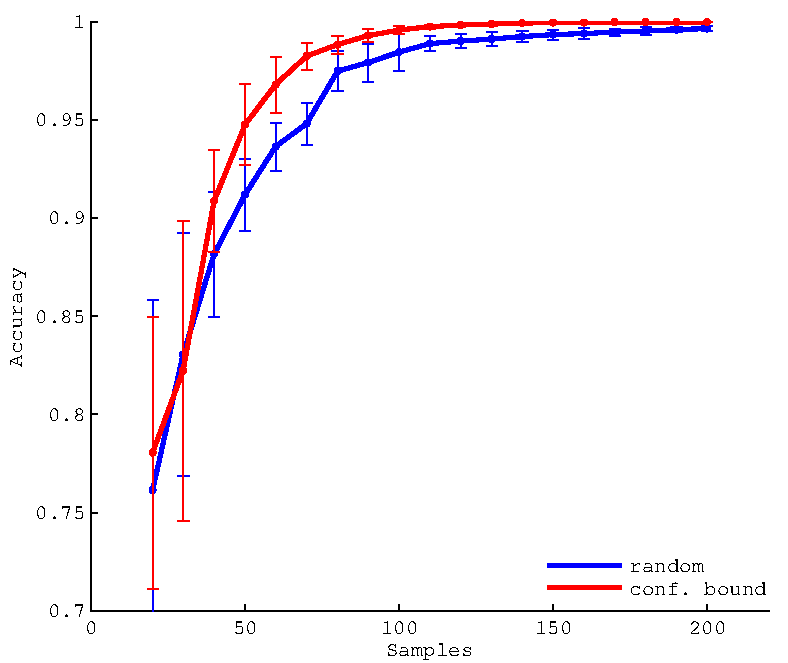
\includegraphics[width=\textwidth]{figures/sin2d_eps_acc}
    \caption{Accuracy}
  \end{subfigure}
  \hfill
  \begin{subfigure}[b]{0.329\textwidth}
    \centering
    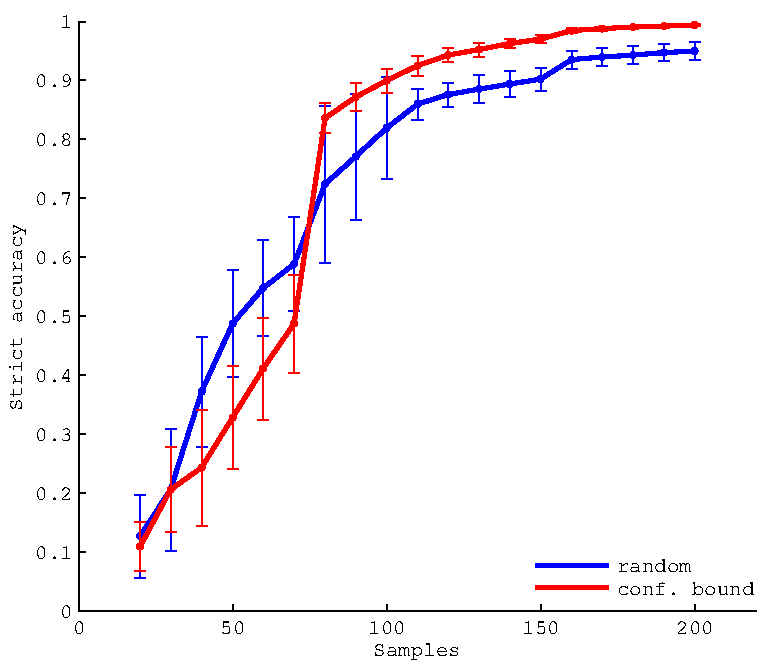
\includegraphics[width=\textwidth]{figures/sin2d_eps_strict_acc}
    \caption{Strict accuracy}
  \end{subfigure}
  \hfill
  \begin{subfigure}[b]{0.329\textwidth}
    \centering
    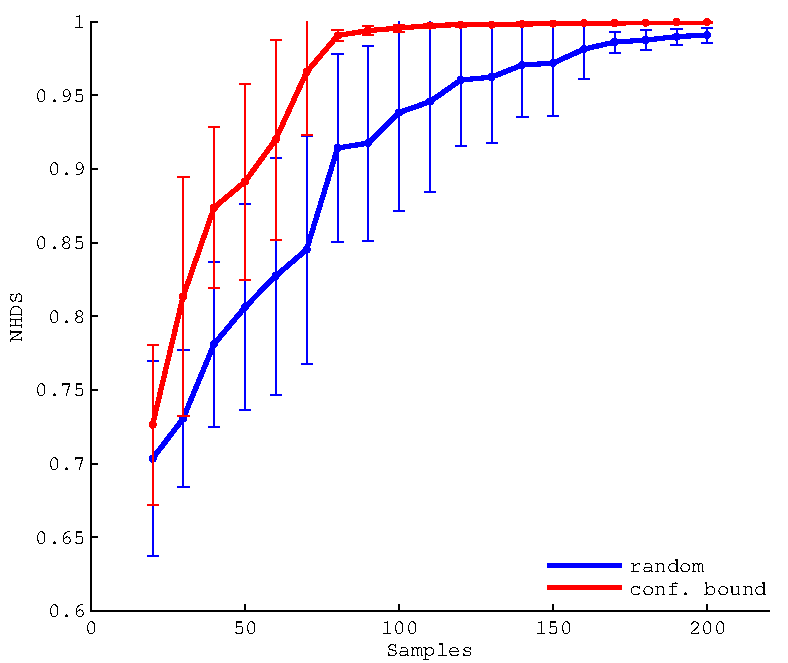
\includegraphics[width=\textwidth]{figures/sin2d_eps_hd}
    \caption{NHDS}
  \end{subfigure}
  \caption{Random and $\epsilon$-optimal conf. bound heuristics evaluated
           on the three metrics for an increasing number of measurements
           (Experiment 1, 20 iterations).}
  \label{fig:sin2d_eval_eps}
\end{figure}

\begin{figure}[h!]
  \begin{subfigure}[b]{0.329\textwidth}
    \centering
    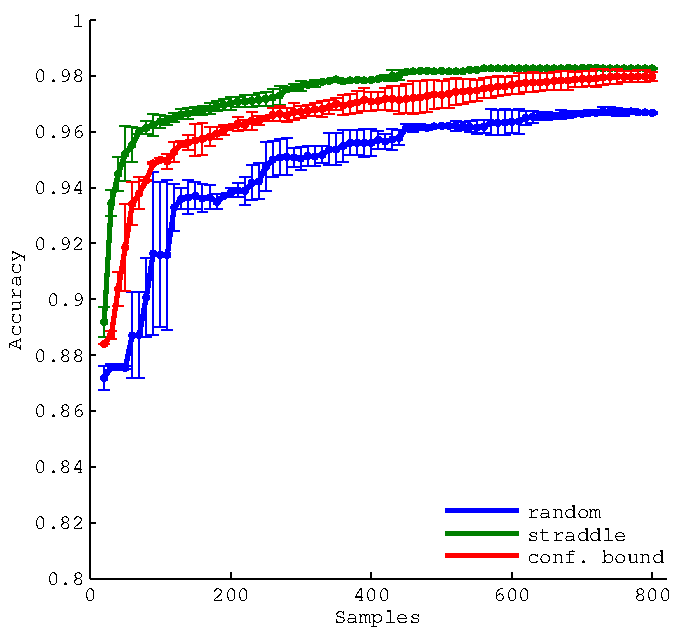
\includegraphics[width=\textwidth]{figures/quake_acc}
    \caption{Accuracy}
  \end{subfigure}
  \hfill
  \begin{subfigure}[b]{0.329\textwidth}
    \centering
    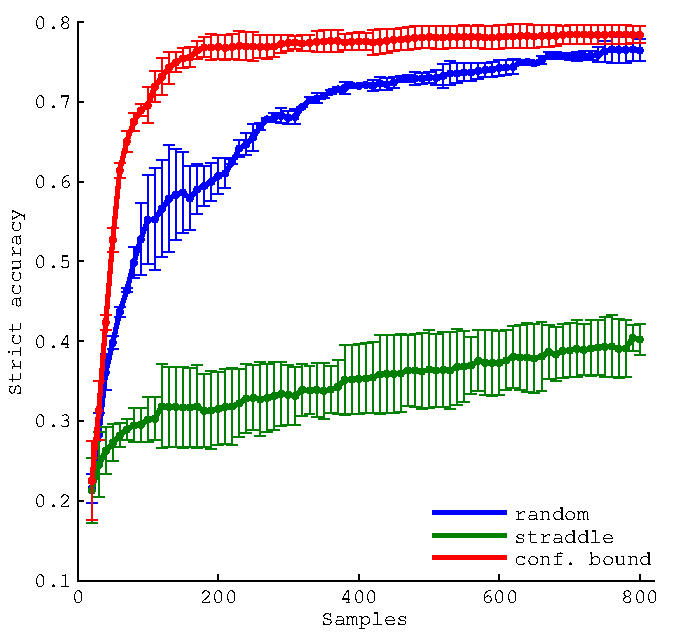
\includegraphics[width=\textwidth]{figures/quake_strict_acc}
    \caption{Strict accuracy}
  \end{subfigure}
  \hfill
  \begin{subfigure}[b]{0.329\textwidth}
    \centering
    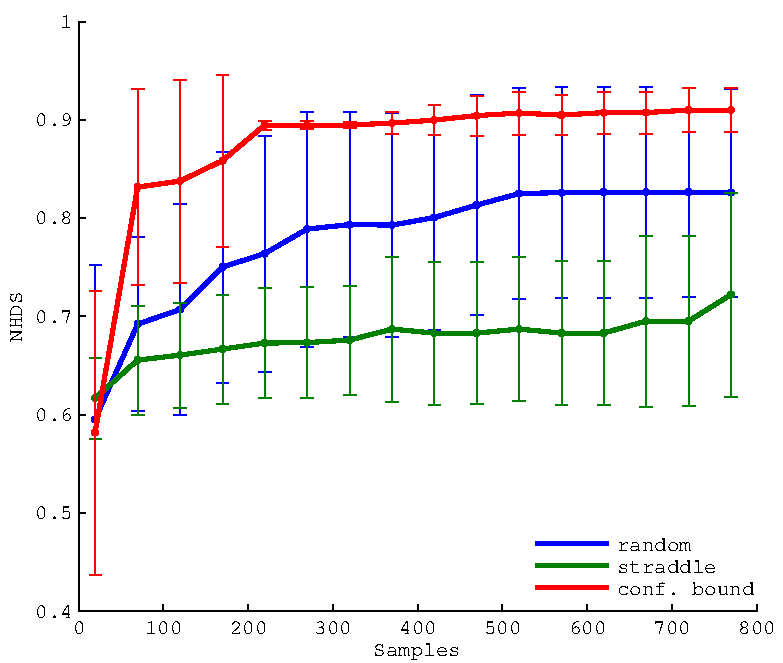
\includegraphics[width=\textwidth]{figures/quake_hd}
    \caption{NHDS}
  \end{subfigure}
  \caption{Random, straddle and conf. bound heuristics evaluated on the three
           metrics for an increasing number of measurements
           (Experiment 2, 20 iterations).}
  \label{fig:quake_eval}
\end{figure}

\subsection{Experiment 2}
In contrast to the previous experiment, the seismographic data of our second
experiment consists of discrete datapoints and, thus, we have no ground
truth contours available. Therefore, we use the inferred model from all
available data samples as the ground truth wherever needed (for plotting and
for evaluating the NHDS).

As before, we evaluate the performance of the algorithm using the three metrics
and the results are shown in \figref{fig:quake_eval}. It is noteworthy that
straddle seems to do marginally better than the conf. bound heuristic
according to accuracy, but is dramatically worse according to the other two
metrics. The reason for this behavior can be explained by referring to
\figref{fig:quake_expl}. In particular, we can see that the measurements of
the straddle heuristic are heavily concentrated on the inferred contour, while
the rest of the region is neglected. As a consequence, the confidence region
does not decrease, which leads to worse strict accuracy scores, and the small
contour on the top right is not detected, which results in worse NHDS scores
(true contours far away from inferred contours are heavily penalized by the
NHDS metric). At the same time, the accuracy score is not affected by the
above observations, because it does not take into account the confidence
region and the effect of a few missclassified samples inside the small
undetected contour is negligible. As can be seen in the same figure,
the conf. bound heuristic explores enough to avoid these problems, but
this has a negative effect on contour accuracy.

The importance of this difference between the two heuristics may depend on
the specific application. In any
case, we can conclude that the straddle heuristic exhibit more exploitative
behavior due to its preference to sample near already inferred contours, which
can lead to oversampling near already accurately determined contours. On the
other hand, the conf. bound heuristic is more exploratory and, in fact, is
similar to maximum variance sampling in cases where the confidence region
cannot be reduced (e.g. due to a bad choice of kernel hyperparameters).


\begin{figure}[tb]
  \begin{subfigure}[b]{0.5\textwidth}
    \centering
    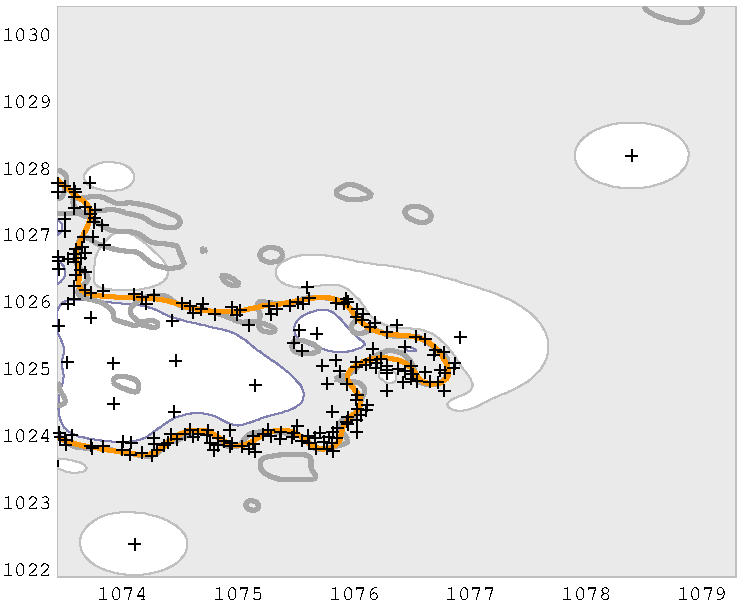
\includegraphics[width=\textwidth]{figures/quake_expl_straddle}
    \caption{Straddle heuristic}
  \end{subfigure}
  \hfill
  \begin{subfigure}[b]{0.5\textwidth}
    \centering
    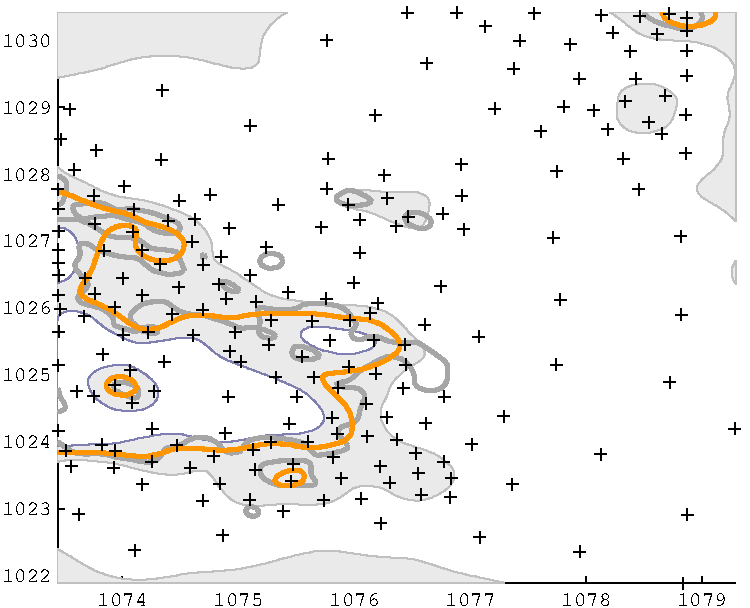
\includegraphics[width=\textwidth]{figures/quake_expl_cb}
    \caption{Conf. bound heuristic}
  \end{subfigure}
  \caption{Example of inferred contours and confidence regions after 200
           measurements on the seismographic data of Experiment 2.}
  \label{fig:quake_expl}
\end{figure}

\section{Conclusion}
We presented a new heuristic for active learning of function contours, which is
based on the confidence bounds provided by Gaussian processes. A tentative
evaluation of the heuristic showed that it is comparable in performance to the
straddle heuristic and may perform better in some cases, depending on the
evaluation metric used. The issues of choosing an appropriate kernel and
a proper evaluation metric require further investigation. It would also be
interesting to evaluate the heuristic
(and its $\epsilon$-optimal extension) to higher-dimensional settings.

\bibliographystyle{plain}
\bibliography{report}

\end{document}
